\documentclass{article}
\usepackage{amssymb,amsfonts,amsmath,amscd,amsthm}
\usepackage{graphicx}
\usepackage{parskip}
\usepackage{color}
\usepackage{bm}
\usepackage{booktabs}
\usepackage{fancyvrb}
\usepackage{booktabs}  %nice tables

\usepackage{tikz}
\usetikzlibrary{positioning}
\usepackage{verbatim}

\tikzset{
  % Specifications for style of nodes:
  base/.style = {
    rectangle,
    rounded corners,
    draw=black,
    text centered
  },
  chain/.style = {
    base,
    minimum width=5.5cm,
    minimum height=2cm,
    node distance=1cm,
    fill=orange!15
  },
  process/.style = {
    base,
    minimum width=1.5cm,
    minimum height=0.75cm,
    node distance=0.25cm,
    fill=blue!15
  },
  vector/.style = {
    rectangle,
    draw=black,
    minimum width=0.42cm,
    minimum height=0.42cm,
    node distance=0.0cm
  },
}

\def\parameter#1{
  \begin{scope}
    \node[vector, fill=green!40, right=of #1.west, xshift=0.11cm] (piece0) {};
    \node[vector, fill=yellow!40, right=of piece0.east, node distance=0cm] (piece1) {};
    \node[vector, fill=red!40, right=of piece1.east, node distance=0cm] (piece2) {};
  \end{scope}
}

\definecolor{dkgreen}{rgb}{0,0.6,0}
\definecolor{gray}{rgb}{0.5,0.5,0.5}
\definecolor{mauve}{rgb}{0.58,0,0.82}

\newcommand{\Quesoweb}{\url{https://github.com/libqueso}}
\newcommand{\Queso}{\texttt{QUESO}}
\newcommand{\QUESOversion}{0.51.0}

\usepackage{listings}          % to include codes using \lstinputlisting
\lstset{
language=c++,                  % choose the language of the code
basicstyle=\ttfamily,          % the size of the fonts that are used for the code
%stringstyle=\ttfamily,
%keywordstyle=\bfseries,       % so funciona com basicstyle=\footnotesize,\ttfamily se eu adicionar \usepackage{bold-extra}
keywordstyle=\color{blue},     % keyword style
commentstyle=\color{dkgreen},  % comment style
stringstyle=\color{mauve},
identifierstyle=\bfseries,
numberbychapter= true,
numberfirstline=false,
% numbers=left,                % where to put the line-numbers
numberstyle=\footnotesize,     % the size of the fonts that are used for the line-numbers
stepnumber=5,                  % the step between two line-numbers. If it is 1 each line will be numbered
numbersep=8pt,                 % how far the line-numbers are from the code
showspaces=false,              % show spaces adding particular underscores
showstringspaces=false,        % underline spaces within strings
showtabs=false,                % show tabs within strings adding particular underscores
tabsize=2,                     % sets default tabsize to 2 spaces
captionpos=b,                  % sets the caption-position to bottom
breaklines=true,               % sets automatic line breaking
breakatwhitespace=false,       % sets if automatic breaks should only happen at whitespace
escapeinside={\%*}{*)},        % if you want to add a comment within your code
morekeywords ={rm,ls},
belowskip = 10pt,              % \medskipamount%\smallskipamount,
aboveskip =10pt,
}

\title{Distributed parameter states in \Queso}
\author{Damon McDougall}

\begin{document}

\maketitle

\section{Introduction}

This document describes the current, serial, state of the parameter vector in
\Queso\ and makes a plan to transition to a distributed state.

\subsection{The current state}

The current state of the parameter vector in \Queso\ is serial.  Parallelism in
\Queso\ presents itself in two ways: 1) independent parallel Markov chains that
execute concurrently; and 2) a mechanism, an MPI communicator, that \Queso\
creates as part of the construction of \lstinline|FullEnvironment| the user can
hand to a forward problem demanding parallelism.  Neither of these parallel
capabilities distribute the parameter vector across multiple processes.  In
other words, each chain's process holds exactly the same parameter vector
value in the likelihood.

Here is some example commented code that executes the current situation:
\begin{lstlisting}
#include <queso/Environment.h>
#include <queso/GslVector.h>
#include <queso/GslMatrix.h>
#include <queso/ScalarFunction.h>
#include <queso/VectorSpace.h>
#include <queso/BoxSubset.h>

using namespace QUESO;

template <class V = GslVector, class M = GslMatrix>
class Likelihood : public BaseScalarFunction<V, M>
{
public:
  Likelihood(const char * prefix,
             const VectorSet<V, M> & domainSet)
    : BaseScalarFunction<V, M>(prefix, domainSet),
      m_env(domainSet.env())
  {
  }

  virtual double lnValue(const V & param) const
  {
    if (m_env.subRank() == 0) {
      std::cout << "Rank 0 param: " << param << '\n';
    }
    else {  // Rank 1
      std::cout << "Rank 1 param: " << param << '\n';
    }

    return 1.0;
  }

  virtual double actualValue(const V&, const V*, V*,
                             M*, V*) const
  {
    return 1.0;
  }

  const BaseEnvironment & m_env;
};

int main(int argc, char ** argv)
{
  // We'll assume the program was executed with
  // mpirun -np 2 and there's only one chain.

  MPI_Init(&argc, &argv);
  FullEnvironment env(MPI_COMM_WORLD, argv[1], "",
                      NULL);
  VectorSpace<> paramSpace(env, "", 2, NULL);
  GslVector min(paramSpace.zeroVector());
  GslVector max(paramSpace.zeroVector());
  min[0] = 0.0;
  min[1] = 0.0;
  max[0] = 1.0;
  max[1] = 1.0;
  BoxSubset<> paramDomain("", paramSpace, min, max);
  Likelihood<> likelihood("", paramDomain);

  GslVector point(paramSpace.zeroVector());
  point[0] = 0.5;
  point[1] = 0.5;
  likelihood.lnValue(point);  // Both ranks print the
                              // same parameter value

  MPI_Finalize();
  return 0;
}
\end{lstlisting}

\subsection{Why we need a distributed state}

There are some issues with a serial parameter vector, and some benefits to
moving to a distributed parameter vector.
\begin{itemize}
  \item There are problems with large parameter vectors (discretized fields)
    that necessitate distribution across multiple processes;
  \item Parallel parameter vector means \Queso\ can leverage existing high
    performance linear algebra packages for better compute resource usage;
  \item High performance linear algebra packages provide better performing
    optimization algorithms we could use before sampling;
  \item The serial implementation requires GSL, and GSL is licensed under the
    GPL.  We have customers at the labs that would like to ship \Queso\ as a
    binary and GPL third-party libraries prevent this from happening.
    \begin{itemize}
      \item A rebuttal to this point might be to use an alternative serial
        implementation with a more liberal license.  This is a reasonable
        suggestion but it doesn't address the first three points.
    \end{itemize}
\end{itemize}

\section{How the future might look}
\subsection{Parameter distribution in parallel}

If the user requests multiple processes per chain, then an approach we might
take is to distribute the parameter across those processes.  In the code
example above, that would mean process 0 sees only the first element of
\lstinline|point| and process 1 sees only the second element.  Here's a
depiction before the change:
%
\begin{center}
  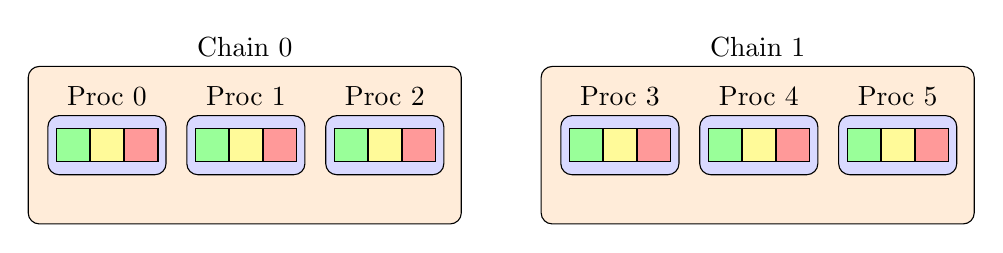
\begin{tikzpicture}
    % Specification of nodes (position, etc.)
    \node[chain, label={Chain 0}] (chain0) at (0, 0)                  {};
    \node[chain, label={Chain 1}, right=of chain0]         (chain1)   {};
    \node[process, label={Proc 0}, right=of chain0.west]   (process0) {};
    \node[process, label={Proc 1}, right=of process0.east] (process1) {};
    \node[process, label={Proc 2}, right=of process1.east] (process2) {};
    \node[process, label={Proc 3}, right=of chain1.west]   (process3) {};
    \node[process, label={Proc 4}, right=of process3.east] (process4) {};
    \node[process, label={Proc 5}, right=of process4.east] (process5) {};
    \parameter{process0}
    \parameter{process1}
    \parameter{process2}
    \parameter{process3}
    \parameter{process4}
    \parameter{process5}
  \end{tikzpicture}
\end{center}
%
And here's what it looks like after the change:
%
\begin{center}
  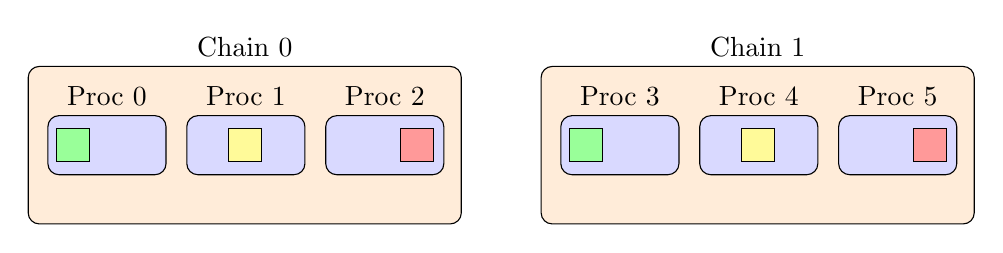
\begin{tikzpicture}
    % Specification of nodes (position, etc.)
    \node[chain, label={Chain 0}] (chain0) at (0, 0)                     {};
    \node[chain, label={Chain 1}, right=of chain0]         (chain1)      {};
    \node[process, label={Proc 0}, right=of chain0.west]   (process0)    {};
    \node[process, label={Proc 1}, right=of process0.east] (process1)    {};
    \node[process, label={Proc 2}, right=of process1.east] (process2)    {};
    \node[process, label={Proc 3}, right=of chain1.west]   (process3)    {};
    \node[process, label={Proc 4}, right=of process3.east] (process4)    {};
    \node[process, label={Proc 5}, right=of process4.east] (process5)    {};
    \node[vector, fill=green!40, right=of process0.west, xshift=0.11cm]  {};
    \node[vector, fill=yellow!40, right=of process1.west, xshift=0.53cm] {};
    \node[vector, fill=red!40, right=of process2.west, xshift=0.95cm]    {};
    \node[vector, fill=green!40, right=of process3.west, xshift=0.11cm]  {};
    \node[vector, fill=yellow!40, right=of process4.west, xshift=0.53cm] {};
    \node[vector, fill=red!40, right=of process5.west, xshift=0.95cm]    {};
  \end{tikzpicture}
\end{center}
%
To maintain compatibility with existing parallel forward problems, \Queso\ will
do all the necessary communication before a likelihood call to organise the
parameter vector.  Inside the likelihood each process belonging to the chain
communicator will receive a serial version of the parameter vector.  Every
process will hold an exact copy of the parameter vector.

The user will not be burdened with providing the mechanism needed to pass a
distributed parameter vector to their forward model.  Therefore, parallel
forward codes that worked with a serial parameter vector will still continue to
work when \Queso\ distributes the parameter vector representation internally.

What about the case where the user needs multiple independent model evaluations
for a single likelihood calculation?  This case arises when there are multiple
experimental data points.  It is reasonable to leverage independent concurrency
for these data points.  Internally, the parameter vector will be distributed
over all processes belonging to the chain communicator. \Queso\ is not
concerned with how these processes are leveraged by the application that
executes the forward model.  For example, if three process are needed for a
single model evaluation and two model evaluations are needed for a single
likelihood evaluation then \Queso\ will distribute the parameter vector over
all six processes.  \Queso\ will do all the necessary MPI communcation before a
likelihood call to ensure that every process belonging to a chain communicator
holds the entire parameter vector.

\subsection{Memory and usability considerations}

We noted in the previous subsection that the parameter vector is distributed
across the processes involved in a chain communicator.

\subsubsection{Usability}

Once a model evaluation needs to be done, it is reasonable to expect that the
model communicator needs the entire parameter vector.  If the parameter vector
is distributed across the entire chain communicator after a call to the
likelihood, the user would be burdened with the point-to-point communication
required to organise the parameter vector for their model, or their model must
be written in such a way that understands and respects \Queso's choice of how
to distributed the parameter vector among the processes in the chain communicator.
This introduces a rather large barrier to entry.

Making each process hold the entire parameter vector (inside the likelihood)
offers a much more user-friendly experience; the user needn't concern
themselves with a potentially burdensome and tricky point-to-point
communication and bookkeeping.  It also offers the possibility of allowing
older forward codes to work with \Queso\ since no code changes would be needed.

\subsubsection{Memory}

It is clear that more memory is required if each process in the chain
communicator holds a copy of the entire parameter vector.  It doesn't seem too
detrimental, however.

In the worst case the user intends to solve an inverse problem in function
space.  In other words, the parameter vector represents a discretised field and
this discretisation may be quite fine.  For inverse problems on function space,
one typically represents the random field by, for example, a truncated KL
expansion.  Inference is done on the coefficients in this expansion.  It is
uncommon to execute an inference at every length scale the discretisation can
represent.  In other words, the inference is done a number of KL coefficients
that is typically much smaller than the number of degrees of freedom offered
by the choice of discretisation.

\subsection{From the user's perspective}

There are a few things to look at:
\begin{enumerate}
  \item The parameter space
  \item The parameter domain
  \item Distributions on the domain (priors)
  \item Interacting with vectors and matrices
  \item The likelihood
\end{enumerate}
These should change as little as possible.

\subsubsection{The parameter space}

At present, the user calls the following to instantiate a parameter space of
dimension 2,
\begin{lstlisting}
MPI_Init(&argc, &argv);
FullEnvironment env(MPI_COMM_WORLD, argv[1], "",
                    NULL);
VectorSpace<> paramSpace(env, "", 2, NULL);
\end{lstlisting}
The parameter space is the same for each chain.  It is only \emph{within} a
chain that the parameter is paritioned.  There is a clear constraint here; the
number of processes belonging to the chain must divide the dimension of the
parameter space.  This might be problematic in the situation where the forward
model needs 10 processes to run quickly for a likelihood evaluation but the
user can't ask for more than 2 processes.

Can we avoid this constraint?  Maybe we allow the user to ask for more
processes per chain and just use a subset of them.  For example, if the user
asks for 10 processes per chain for the forward model evaluation then \Queso\
would also ask for how many of those the parameter should be distributed over.

\subsubsection{The parameter domain}

For a \lstinline|BoxSubset|, which is the most common domain, the user calls
\begin{lstlisting}
BoxSubset<> paramDomain("", paramSpace, min, max);
\end{lstlisting}
The parameter space is already partitioned and \lstinline|min| and
\lstinline|max| belong to the parameter space.  Everything is already set up
for the parameter domain and nothing needs to be done here from the user's
perspective.

What about other domains?  Another common domain is the
\lstinline|ConcatenatedSubset|.  What about user-defined domains?

\subsubsection{Distributions on partitioned domains}

As an example, a user might construct a Gaussian distribution for the prior.
The user calls
\begin{lstlisting}
GaussianVectorRV<> prior("", paramDomain, mean,
                         covariance);
\end{lstlisting}
From the user's perspective, nothing would need to change.  The mean belongs
to the already-partitioned parameter vector space, and so does the covariance
matrix.

Any distributions that rely on vectors or matrices for construction will lie
in the already-partitioned space and the user will see no changes in their
statistical application.

\subsubsection{Interacting with vectors and matrices}

We mentioned briefly that nothing special needs to be done to set up vector
spaces and domains.  We saw that these may depends on vectors and matrices the
user must construct, and we explore that interaction here.

The user may interact with vectors in two different ways: 1) the user interacts
with a serial vector; or 2) the user interacts with a parallel vector.  The
dimension of the vector space (integer passed in the \lstinline|VectorSpace<>|
constructor) is the global dimension.  This is important to note, because
\Queso\ will use it to determine which of the two interactions are used.
If the serial vector interaction is used, then the length of each local vector
is exactly the same as the global dimension.  If the parallel vector
interaction is used, then the sum of each of the local vector lengths is equal
to the global dimension.  If the user chooses to interact with a parallel
vector then they are explicitly defining a partioning of that vector among
processes in the chain communicator.  \Queso\ will respect this partioning
when doing, for example, matrix-vector operations.  If the user interacts with
a serial vector then \Queso\ will parition it automatically before doing
matrix-vector operations.  This code
\begin{lstlisting}
// Serial vector interaction
GslVector<> v(paramSpace.zeroVector());
v[0] = 1.0;
v[1] = 2.0;
\end{lstlisting}
will set global (and local) index 0 on process 0 and global (and local) index 0
on prcoessor 1.  Both processes belonging to the chain hold the 2-vector
$(1, 2)$.  This code
\begin{lstlisting}
// Parallel vector interaction
Map map(2, 0, env.subComm());
GslVector<> v(env, map);

if (env.subRank() == 0) {
  v[0] = 1.0;
}
else if (env.subRank() == 1) {
  v[0] = 2.0;
}
\end{lstlisting}
will set local index 0 on process 0 and local index 0 on process 1.  Local
index 0 on processor 1 should map to global index 1 for \lstinline|v|.  Process
0 holds the 1-vector $(1)$ and process 1 holds the 1-vector $(2)$.  Together
they represent the partitioned 2-vector $(1, 2)$.

Interacting with matrices has a similar story.  The user can interact with a
serial matrix and \Queso\ will partition it behind the scences, or the user
can choose a partitioning and \Queso\ will respect the user's choice.  This
code
\begin{lstlisting}
// Parallel matrix interaction
GslMatrix<> A(env, map, 2);

if (env.subRank() == 0) {
  A(0, 0) = 1.0;
  A(0, 1) = 0.5;
}
else if (env.subRank() == 1) {
  A(0, 0) = 0.5;
  A(0, 1) = 1.0;
}
\end{lstlisting}
will set local row index 0 on process 0 and local row index 0 on process 1.
Local row index 0 on process 1 should map to global row index 1 for
\lstinline|A|.

\subsubsection{The likelihood}

This part, from the user's perspective, doesn't change.  Inside the call to
\lstinline|lnValue| the parameter \lstinline|param| (from the first code
example) doesn't change.  It is a serial vector; each process belonging to the
chain communicator has an exact copy of the global vector \lstinline|param|.

\subsection{From \Queso's perspective}

\end{document}
